\maketitle
\setcounter{page}{1}
\tableofcontents
\newpage
\pagenumbering{arabic}
\section{Theorie}
Der Zeeman-Effekt tritt auf, wenn Atome einem externen Magnetfeld unterworfen
werden. Dadurch wird die Entartung der Energieniveaus in der Quantenzahl $m$
aufgehoben, sodass die diese Energieniveaus aufspalten. \\
\\
Zur Berechnung der Wechselwirkung der Drehimpulse und der magnetischen Momente
untereinander, müssen die Drehimpulse eines Hüllenelektrons betrachtet werden, also
der Bahndrehimpuls $\vec{l}$ und der Spin $\vec{s}$. Das magnetische Moment
des Drehimpulses ist definiert nach
\begin{equation}
  \vec{\mu}_l = -\mu_B \, \frac{\vec{l}}{\hbar} = -\mu_B \, \sqrt{l(l+1)} \ \vec{l}_e
  \label{eqn:1}
\end{equation}
mit dem magnetischen Moment
\begin{equation*}
  \mu_B = -\frac{1}{2} \, \symup e_0 \, \frac{\hbar}{\symup m_0} \, ,
\end{equation*}
dem Einheitsvektor $\vec{l}_e$ in $\vec{l}$ Richtung und mit Elementarladung und
Ruhemasse des Elektrons.
Aus dem Spin-Gerlach-Experiment folgt das Analogon für den Spin
\begin{equation}
  \vec{\mu}_s = - \symup g_s \, \frac{\mu_B}{\hbar} \, \vec{s}
  = - \symup g_s \, \mu_B \, \sqrt{s(s+1)} \ \vec{s}_e
  \label{eqn:2}
\end{equation}
mit dem \textsc{Landé-Faktor} des Elektrons $\symup g_s$, welcher ungefähr den
Wert 2 besitzt. Wie aus \eqref{eqn:1} und \eqref{eqn:2} ersichtlich, ist damit
$\vec{\mu}_s$ entwa doppelt so groß wie $\vec{\mu}_l$. Dies wird als \textbf{magnetomechanische
Anomalie des Elektrons} bezeichnet. Nun werden, wie bereits erwähnt, die Wechelwirkungen
der Drehimpulse und magnetischen Momente untereinander und miteinander behandelt.
Da diese aber im Allgemeinen sehr unübersichtlich sind, werden zwei Grenzfälle betrachtet:
\begin{itemize}
  \item \textbf{Niedrige Kernladungszahl}:
  Die Wechselwirkung zwischen den Bahndrehimpulsen ist so dominant, dass sich
  durch Addition ein Gesamtdrehimpuls $\vec{L}$ der Hülle aus diesen bildet. Die
  Bahndrehimpulse von abgeschlossenen Schalen sind dabei stets 0 und fließen somit
  nicht in den Gesamtdrehimpuls ein. $\vec{L}$ ist dabei quantisiert, und zwar
  gibt es nur Gesamtdrehimpulse, deren Quantenzahl ganzzahlig ist. Die Terme zu den
  Quantenzahlen 0, 1, 2 und 3 heißen S-, P-, D- und F-Terme. Der Gesamtdrehimpuls
  hat ebenfalls ein zugehöriges magnetisches Moment, welches sich aus \eqref{eqn:1}
  zu
  \begin{equation}
    |\vec{\mu}_L| = \mu_B \, \sqrt{L(L+1)}
    \label{eqn:3}
  \end{equation}
  ergibt. Auch für den Spin gibt es einen Gesamtspin, analog zum Bahndrehimpuls,
  mit dem Unterschied, dass für die Quantisierung $\frac{N}{2}, \frac{N}{2} - 1, ...,
  \frac{1}{2}, 0$ (Mit $N$ als Gesamtzahl der Elektronen in unabgeschlossenen Schalen) gilt.
  Analog zu \eqref{eqn:3} gilt für das magnetische Moment des Gesamtspins
  \begin{equation}
    |\vec{\mu}_s| = \symup g_s \mu_B \, \sqrt{S(S+1)} \, .
    \label{eqn:4}
  \end{equation}
  Unter der Vorraussetzung, dass das angelegte externe Magnetfeld kleiner als ungefähr
  \SI{10}{\tesla}, koppeln Gesamtspin $\vec{S}$ und Gesamtdrehimpuls $\vec{L}$ zum Gesamtdrehimpuls
  $\vec{J} = \vec{L} + \vec{S}$ der Elektronenhülle. Dies nennt sich \textbf{LS-Kopplung}.
  Für den Versuch wird diese Kopplungsart angenommen. Die Quantenzahl des Gesamtdrehimpulses
  ist entweder halb- oder ganzzahlig, abhängig von S.
  \item \textbf{Hohe Kernladungszahl}:
  In diesem Fall ist die Wechselwirkung zwischen Spin und Bahndrehimpuls eines
  Elektrons dominant gegenüber der Wechselwirkung der Größen untereinander. Somit
  existiert kein Gesamtdrehimpuls und Gesamtspin, lediglich der Gesamtdrehimpuls
  \begin{equation*}
    \vec{J} = \sum_i \ \vec{l}_i + \vec{s}_i
  \end{equation*}
  der Hülle existiert noch.
\end{itemize}
Nun wird die

\section{Auswertung}
\subsection{Eichung des B-Feldes}
Die Messwerte sowie eine graphische Darstellung mit Fit sind in Abbildung \ref{A_Abb:1}
dargestellt. Der Fit wurde nach least-squares durch die Funktion $\textsc{polyfit}$
aus dem $\textsc{Python}$\footnote{Version: 3.6.3} Paket
$\textsc{numpy}$\footnote{Version: 1.13.3} mit einem Polynom 3. Grades erstellt.

\begin{figure}[h!]
  \centering
  \subcaptionbox{Messwerte.}[0.20\textwidth]{
  \centering
  \begin{tabular}{c c}
    \toprule
    $I / \si{\ampere}$ & $B / \si{\milli\tesla}$ \\
    \midrule
    0 & 5 \\
    1 & 64 \\
    2 & 139 \\
    3 & 191 \\
    4 & 237 \\
    5 & 308 \\
    6 & 363 \\
    7 & 423 \\
    8 & 486 \\
    9 & 533 \\
    10 & 599 \\
    11 & 662 \\
    12 & 720 \\
    13 & 770 \\
    14 & 821 \\
    15 & 870 \\
    16 & 915 \\
    17 & 949 \\
    18 & 985 \\
    19 & 1006 \\
    20 & 1032 \\
    \bottomrule
  \end{tabular}
  }
  \subcaptionbox{Grafische Darstellung mit Regression.}[0.78\textwidth]{
  \centering
  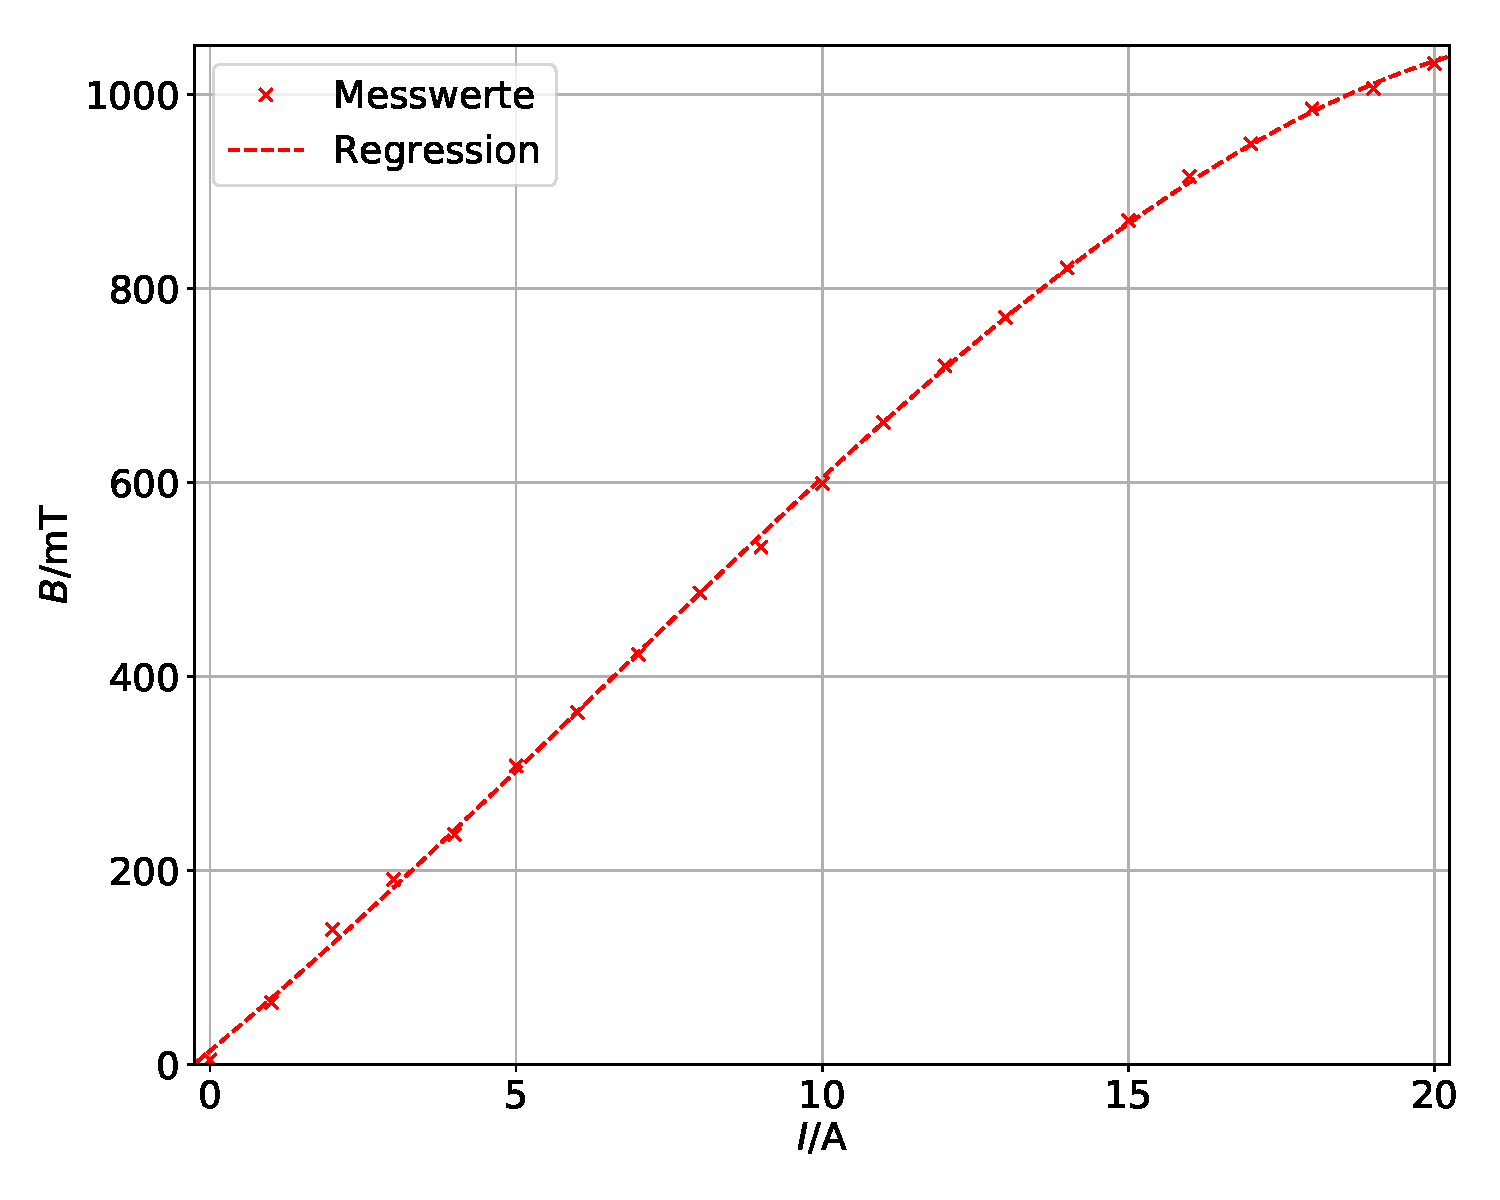
\includegraphics[width=0.78\textwidth]{B_Feld.pdf}
  }
  \caption{Magnetfeldeichung.}
  \label{A_Abb:1}
\end{figure}

Die Fitparameter mit Fehlern lauten:
\begin{align}
\begin{split}
  a_3 &= \SI{-0.072(9)}{\milli\tesla\per\cubic\ampere}\\
  a_2 &= \SI{1.350(269)}{\milli\tesla\per\square\ampere}\\
  a_1 &= \SI{52.760(2284)}{\milli\tesla\per\ampere}\\
  a_0 &= \SI{14.007(5145)}{\milli\tesla}.
  \label{A_eq:1}
\end{split}
\end{align}
Mit den Werten in \eqref{A_eq:1} folgt also als genäherte Feldstromstärke - Magnetfeld
- Beziehung:
\begin{equation}
  B(I) = a_3 \cdot I^3 + a_2 \cdot I^2 + a_1 \cdot I + a_0
\end{equation}



\newpage
\nocite{*}
\printbibliography
